% --
% raw audio

\section{Raw Audio Waveforms}\label{sec:signal_raw}
Physical acoustic waves can be recorded by microphones, translating mechanical vibrations to electrical signals. 
Those electrical signals can be further stored in \emph{audio files} using a specific audio format, for example the \texttt{.wav} format.
Apart from any compression technique, the most important storage details are the bit resolution, for instance, \SI{24}{\bit} floating point and the sample rate $f_s$.
The sample rate defines the frequency range a continuous audio signal can be stored in discrete representation.
The limit of the frequency range is given by the Nyquist-Shannon sampling theorem, where the maximum frequency of the signal $f_{x_{max}}$ should not exceed the half of the sampling frequency
\begin{equation}\label{eq:signal_raw_nyquist}
  f_{x_{max}} < \frac{f_s}{2}
\end{equation}
in order to avoid aliasing effects in the sampled signal.
For that reason the compact disc (CD) format uses a sampling frequency of \SI{44.1}{\kilo\hertz}, resulting in a maximum signal frequency of \SI{22.05}{\kilo\hertz}, exploiting the fact that humans do not hear above \SI{20}{\kilo\hertz} frequencies.
Although it is affordable to go far beyond those \SI{44.1}{\kilo\hertz} in the application of speech signals. 
For instance, the telephone systems use a sampling rate of \SI{8}{\kilo\hertz}.
Speech signals usually do not require such a high sampling frequency to result in sufficient quality and being perceived as understandable.
Music on the other hand, requires a high sampling frequency for being enjoyable to listen to.

With the sampling frequency known, a discrete time signal of an audio recording $\bm{x} \in \R^n$ can be expressed in vector notation by
\begin{equation}\label{eq:signal_raw_x}
  \bm{x} = [x_1, x_2, \dots, x_n]^T
\end{equation}
with a total number of $n$ samples.
The recorded audio files provided in the speech command dataset \cite{Warden2018}, which are further applied in the experiments in \rsec{exp}, are sampled with a sampling rate of \SI{16}{\kilo\hertz} and usually have a time duration of \SI{1}{\second} apart from some individual shorter files.

For evaluation and visualization purpose, the author of this thesis has recorded examples of the speech commands \{\enquote{left}, \enquote{right}, \enquote{up}, \enquote{down}, \enquote{go}\} with a simple consumer Lavalier microphone.
One example of each of those speech commands is contained in the showcase examples, visualized in \rfig{signal_raw_showcase} in raw audio format, and will be used to illustrate the whole feature extraction process in the following sections.
\begin{figure}[!ht]
  \centering
    \subfigure[left]{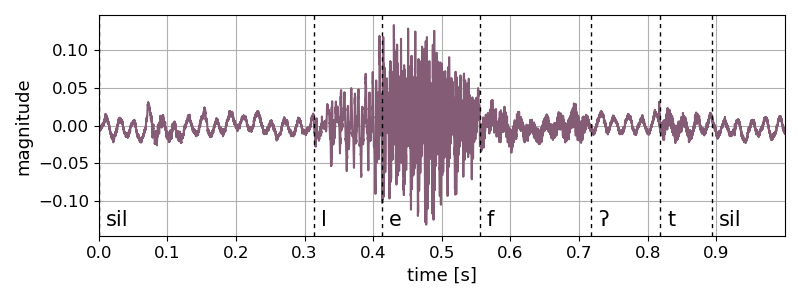
\includegraphics[width=0.45\textwidth]{./3_signal/figs/signal_raw_showcase_left0.png}}
    \quad
    \subfigure[right]{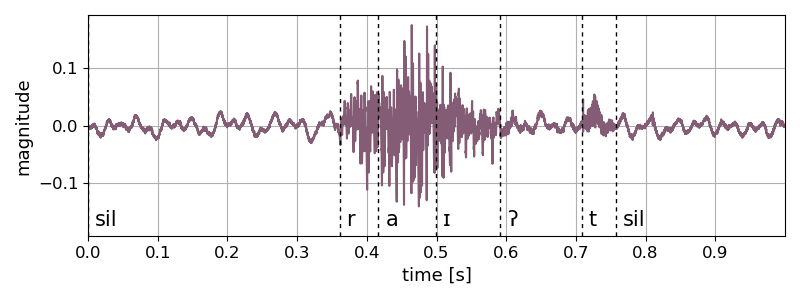
\includegraphics[width=0.45\textwidth]{./3_signal/figs/signal_raw_showcase_right0.png}}
    \subfigure[up]{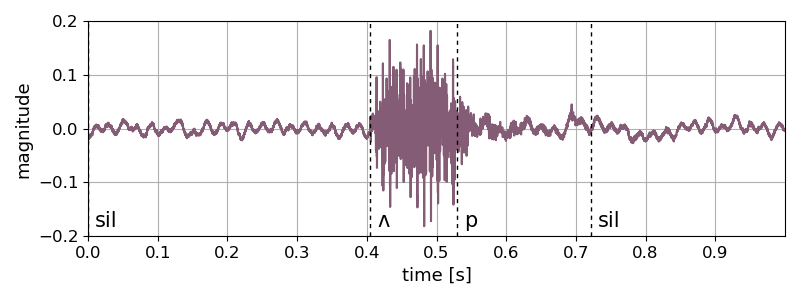
\includegraphics[width=0.45\textwidth]{./3_signal/figs/signal_raw_showcase_up0.png}}
    \quad
    \subfigure[down]{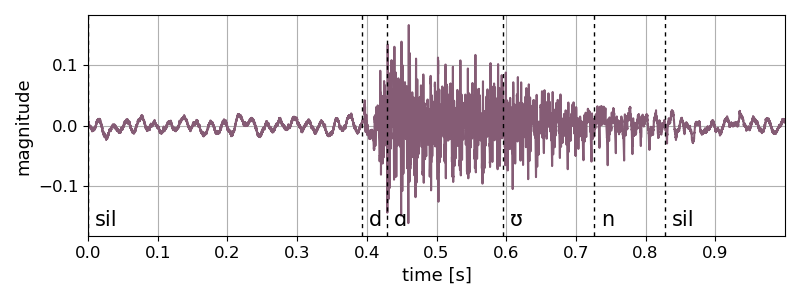
\includegraphics[width=0.45\textwidth]{./3_signal/figs/signal_raw_showcase_down0.png}}
    \subfigure[go]{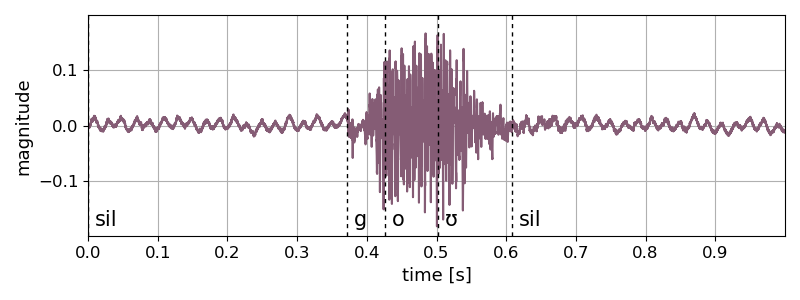
\includegraphics[width=0.45\textwidth]{./3_signal/figs/signal_raw_showcase_go0.png}}
  \caption{Self recorded showcase examples of speech commands presented in the raw audio waveform format. Phoneme onsets are marked by vertical dashed lines.}
  \label{fig:signal_raw_showcase}
\end{figure}
\FloatBarrier
\noindent
From the shown recordings it can be estimated how long a speech command out of this vocabulary may take in terms of duration.
The observation of those examples suggests that usually a duration of \SI{1}{\second} is too much.
The pronunciation of words can of course deviate strongly in duration.
But usually when using commands words, it is preferred to speak shortly and well pronounced.
When a time interval of \SI{500}{\milli\second} is used to capture a speech command (this time interval is used in the feature extraction stage in the experiments), it might happen that not every phoneme of the spoken words is captured.
Often this might occur for words with glottal stops before consonants, for example, the phoneme \enquote{t} in \enquote{left} or \enquote{right}, hence the input features may only contain information of the first phonemes and miss the \enquote{t}.
However, since KWS is limited by its vocabulary and no similar words are contained within, it should be no problem in distinguishing them.

Another important aspect is to detect an appropriate onset (beginning of the keyword) position on the time axis of the speech signal.
This is useful to fit the keyword examples into a smaller time interval that should represent most of the keyword's information within.
In \rfig{signal_raw_showcase} it is easy to spot the beginning and ending of the showcase examples but usually not all recordings are as clean as those.
There might be a large noise floor, imminent background sound, or cut off signals so that the detection of the right onset position for the \SI{500}{\milli\second} time interval within the \SI{1}{\second} recordings is not always accurate.
The applied onset detection is therefore separately discussed in \rsec{signal_onset}.

Moreover, it is worth mentioning that the value range of audio recordings heavily depends on the used microphone, amplifier, and post processing stage.
It is therefore strongly recommended to normalize all recordings to a defined value range before applying the feature extraction.
The normalization can be achieved, for instance, by dividing each sample of the signal by the infinity norm of the whole signal as follows:
\begin{equation}
  \bm{x} \gets \frac{\bm{x}}{\norm{\bm{x}}_\infty}
\end{equation}
so that the maximum or minimum value of $\bm{x}$ corresponds to either $+1$ or $-1$ and the signal range is defined between $[-1, 1]$.